\subsection{Long-Term Temperature Trends}

To investigate the long-term changes in climate, the maximum, minimum, and mean temperatures were analyzed over the period 1850--2024. Linear fits were applied to estimate the overall rate of temperature change in both individual stations and the combined Swedish dataset.


Figure \ref{fig:lund_maxmin} and \ref{fig:lund_mean} shows the temperature trends for the Lund station. The results show an increase in maximum temperature and a decrease in minimum temperature over the studied period. This implies that while summers have become warmer, winters or night-time temperatures have become colder. Consequently, the annual temperature range has widened, suggesting stronger variability. The mean annual temperature, however, still shows a slight positive linear trend, consistent with an overall gradual warming of approximately one degree per century.

\begin{figure}[H]
    \centering
%    \begin{subfigure}[b]{0.48\textwidth}
        \centering
        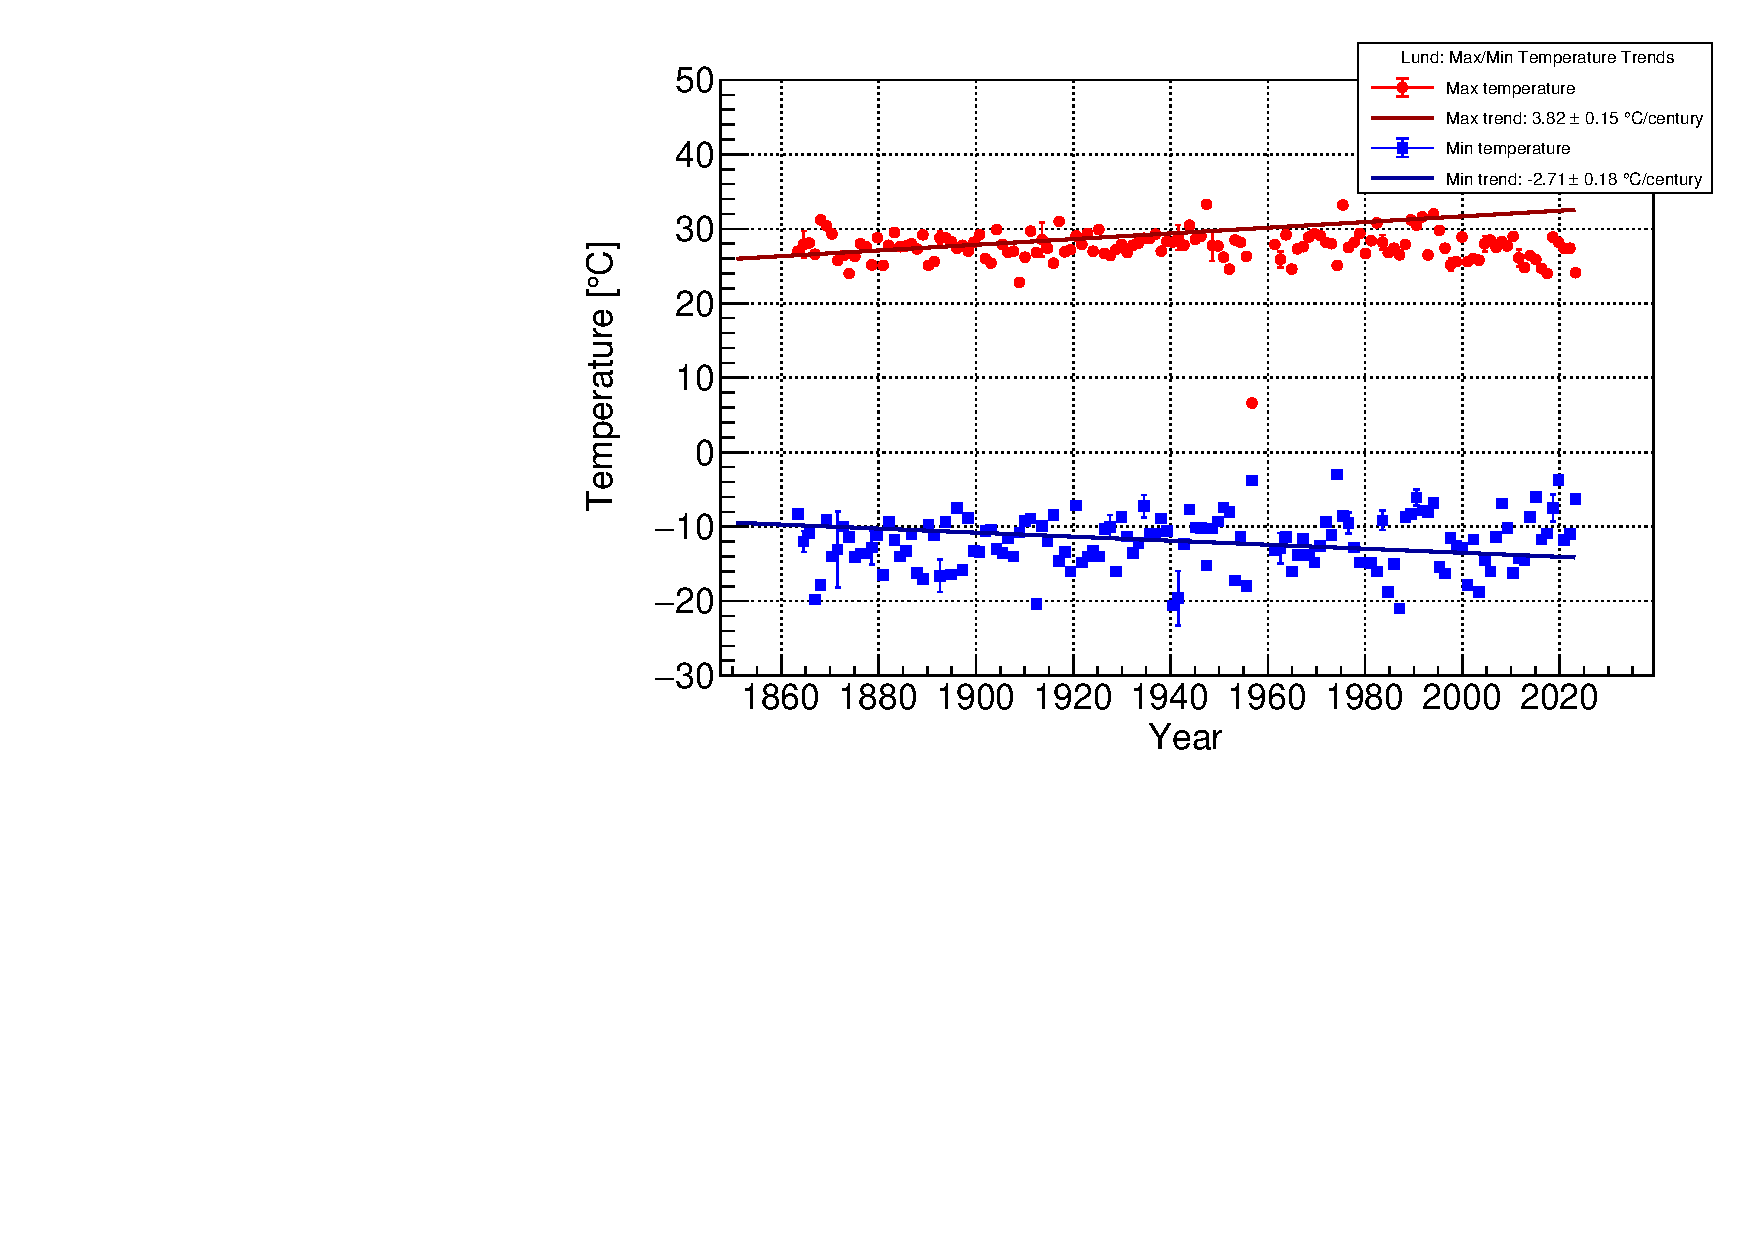
\includegraphics[width=0.9\textwidth]{plots/max_min_temps/Lund_max_min_trends.pdf}
        \caption{Long-term temperature trends at the Lund station (1850--2024). 
    Linear fits are shown for maximum and minimum temperatures. The fits shows an increase in maximmum annual temperature of about four degrees per century and a decrease in minimun annual temperature of about three degrees per century.}
        \label{fig:lund_maxmin}
%    \end{subfigure}
\end{figure}
%    \hfill
\begin{figure}[H]
%    \begin{subfigure}[b]{0.48\textwidth}
        \centering
        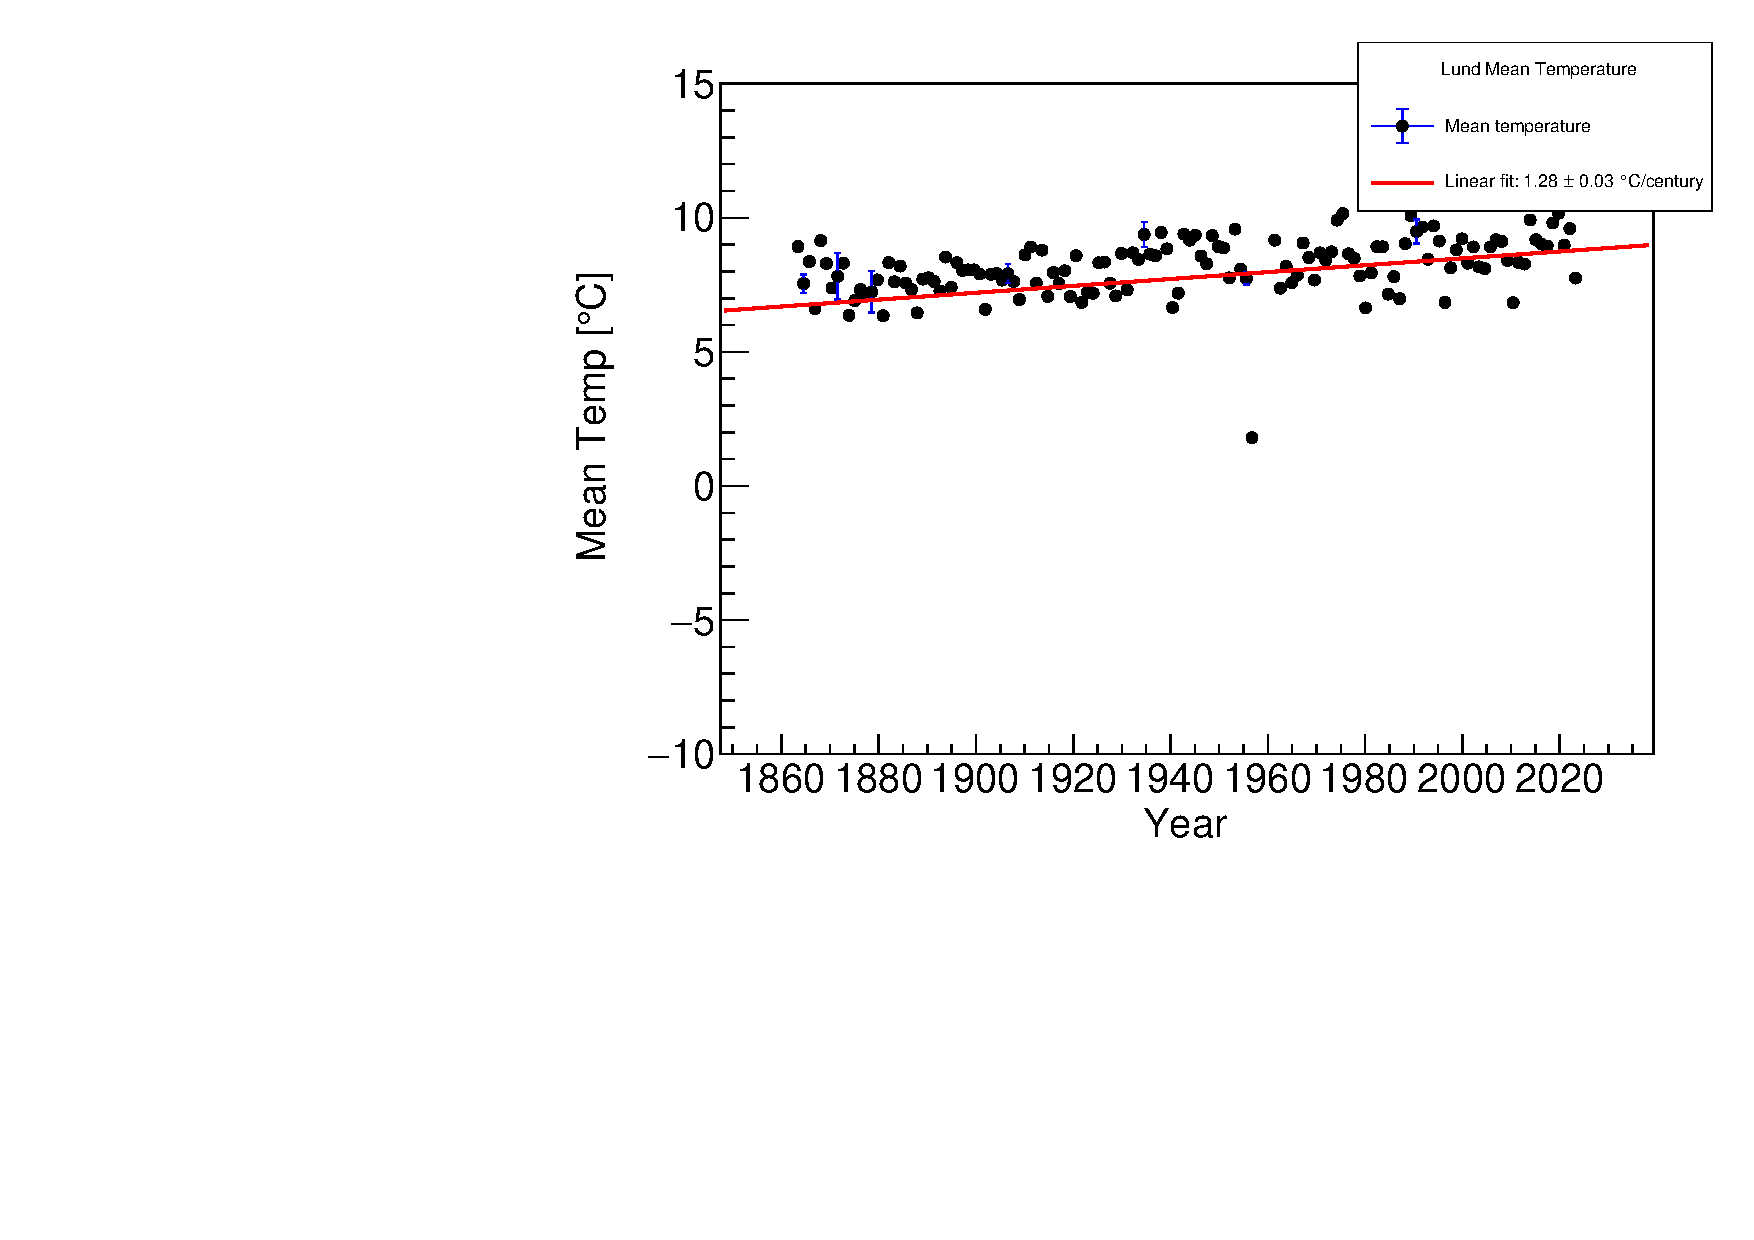
\includegraphics[width=0.9\textwidth]{plots/mean_temps/Lund_mean_trend.pdf}
        \caption{Long-term temperature trends at the Lund station (1850--2024). 
    Linear fits are shown for mean annual temperature. The fit shows an increase in temperature of about 1 degree per century.}
        \label{fig:lund_mean}
%    \end{subfigure}
%    \caption{Long-term temperature trends at the Lund station (1850--2024). 
%    Linear fits are shown for maximum, minimum, and mean temperatures.}
%    \label{fig:lund_trends}
\end{figure}


The results from multiple stations were combined to represent the general temperature trend in Sweden, as shown in Figure \ref{fig:sweden_trend}. The combined data show a positive trend, with average temperatures increasing by about one degree per century. The consistency across different stations indicates that the observed warming is not localized, but reflects a general national trend.

\begin{figure}[H]
    \centering
    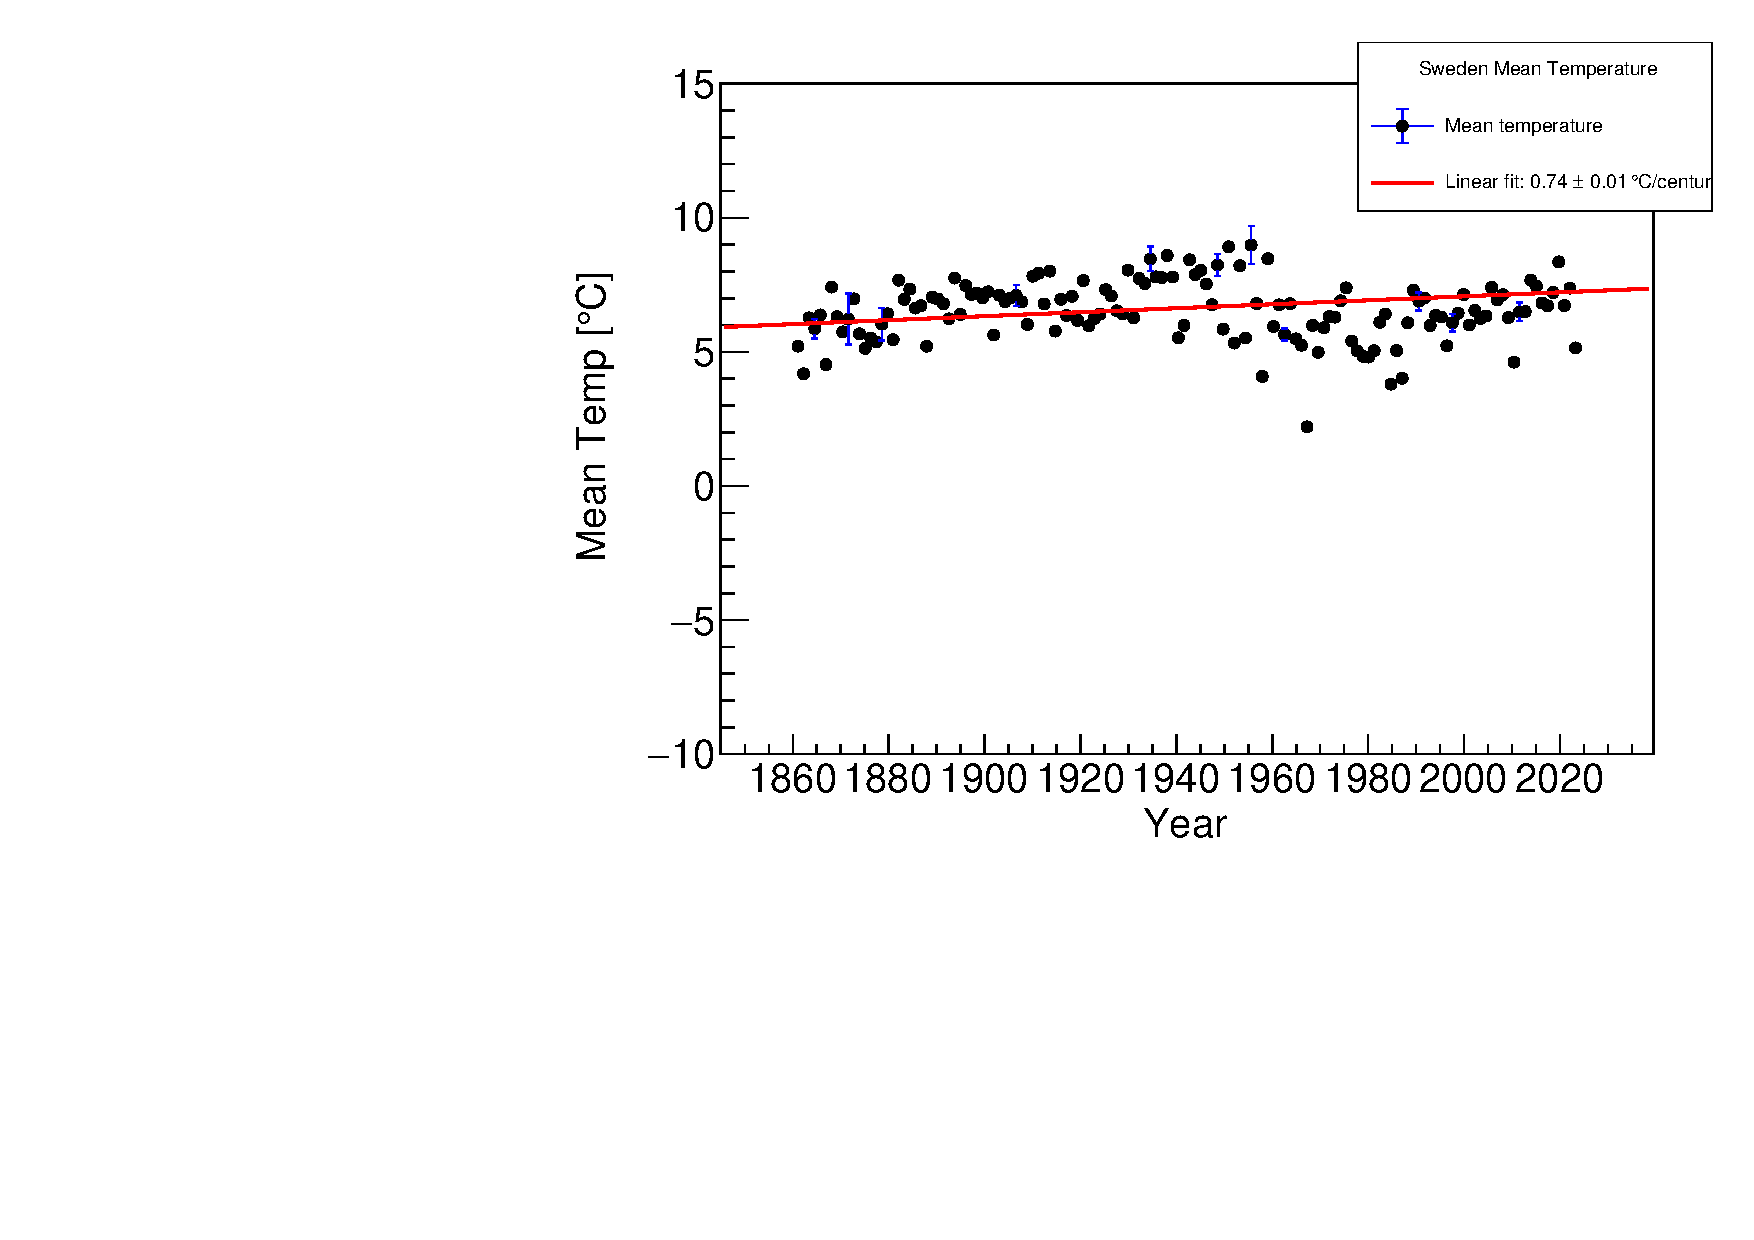
\includegraphics[width=0.9\textwidth]{plots/mean_temps/Sweden_mean_trend.pdf}
    \caption{Combined long-term temperature trend for Sweden based on multiple stations (1850--2024). The fit shows an overall warming of about one degree per century.}
    \label{fig:sweden_trend}
\end{figure}

\subsubsection{Discussion}

The temperature analysis for both the Lund station and the combined Sweden dataset shows a clear climate impact on the temperature from the mid-19th century to the present day. The linear fits for mean, maximum, and minimum temperatures all indicate slopes toward the extremes, suggesting that Sweden has experienced a gradual change in temperature over the past 170 years.

While the warming trend is consistent with global climate change observations, some local variations are visible. Lund, for example, shows slightly larger fluctuations and a stronger trend in minimum temperature, which may reflect urban heat effects or regional climate differences. The national average tends to smooth out such variations, giving a clearer picture of the overall climate trend in Sweden.

It is important to note that a linear approximation is a simplification. Temperature evolution is influenced by many factors, including natural variability, solar activity, oceanic cycles, and greenhouse gas emissions. Limited resolution and occasional data gaps, especially in older records, also introduce uncertainty in the estimated trends.

\subsubsection{Conclusion}

The analysis confirms a significant impact on the temperature trend across Sweden, with both maximum and minimum annual temperatures going toward the extremes since 1850. The results align with broader global climate observations and provide clear evidence of regional climate change effects. We can see that Sweden will experience colder winters and warmer summers, with the average temperature increasing.

For future work, more detailed modeling could include seasonal decomposition or non-linear fits to capture shorter-term oscillations and long-term variability. Combining temperature data with other meteorological parameters such as precipitation, solar radiation, or atmospheric CO$_2$ concentration would also allow for a clearer view of the driving factors behind these trends.

Overall, the study demonstrates how historical climate data and modern analysis tools like ROOT can be used to visualize and quantify long-term climate evolution in a clear and reproducible way.
